\chapter{Background}
\label{ch:background}
*** Put in a description of the PackBot, Talon and Urbot. Talk about JAUS and MOCU a little bit. Discuss more about how the robots are used by EOD. Include that for robots to drive around on their own all they require is an estimate of where they are, a path to follow, a controller to determine the actuator outputs and motor controllers to perform the controller outputs. ***

*** It might be best to have more of a description of the actual problem here along with a description of the testing area. ***

\section{Small Unmanned Ground Vehicles}
\label{sec:smallugvs}
The \href{http://www.irobot.com/sp.cfm?pageid=171}{PackBot} is manufactured by iRobot and can be seen in Figure \ref{fig:packbot}. *** Add more. ***

\begin{figure}[ht!]
	\centering
	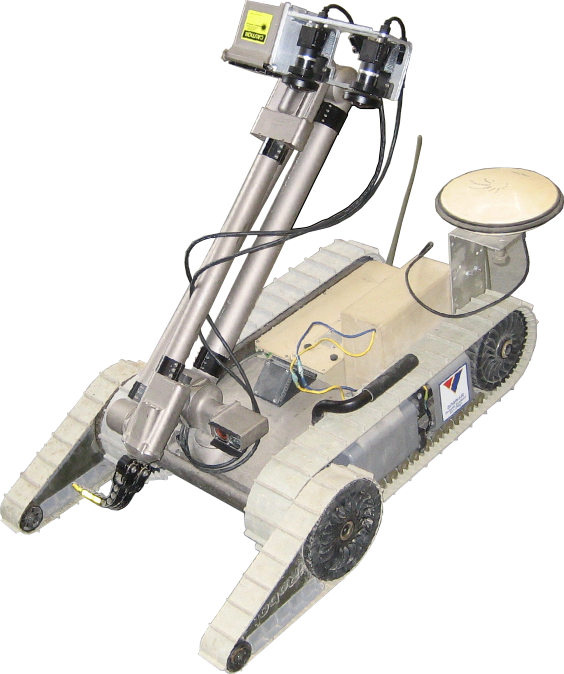
\includegraphics[width=.3\textwidth]{images/packbot}
	\caption{Packbot.}
	\label{fig:packbot}
\end{figure}

The \href{http://www.foster-miller.com/lemming.htm}{Talon} is manufactured by Foster Miller. *** Add more. ***

The \href{http://www.spawar.navy.mil/robots/land/mprs/mprs.html}{Urbot} is an experimental prototype of a small UGV developed by SSCPAC and is shown in Figure \ref{fig:urbot}. *** Add more. Get a picture with better angles like for the PackBot so that the axes can be put in properly. Also, get that picture with everything closed up so its guts aren't hanging out all over the place. ***

*** Say that each of the robots has a standard sensor suite and list what those sensors are. ***

\begin{figure}[ht!]
	\centering
	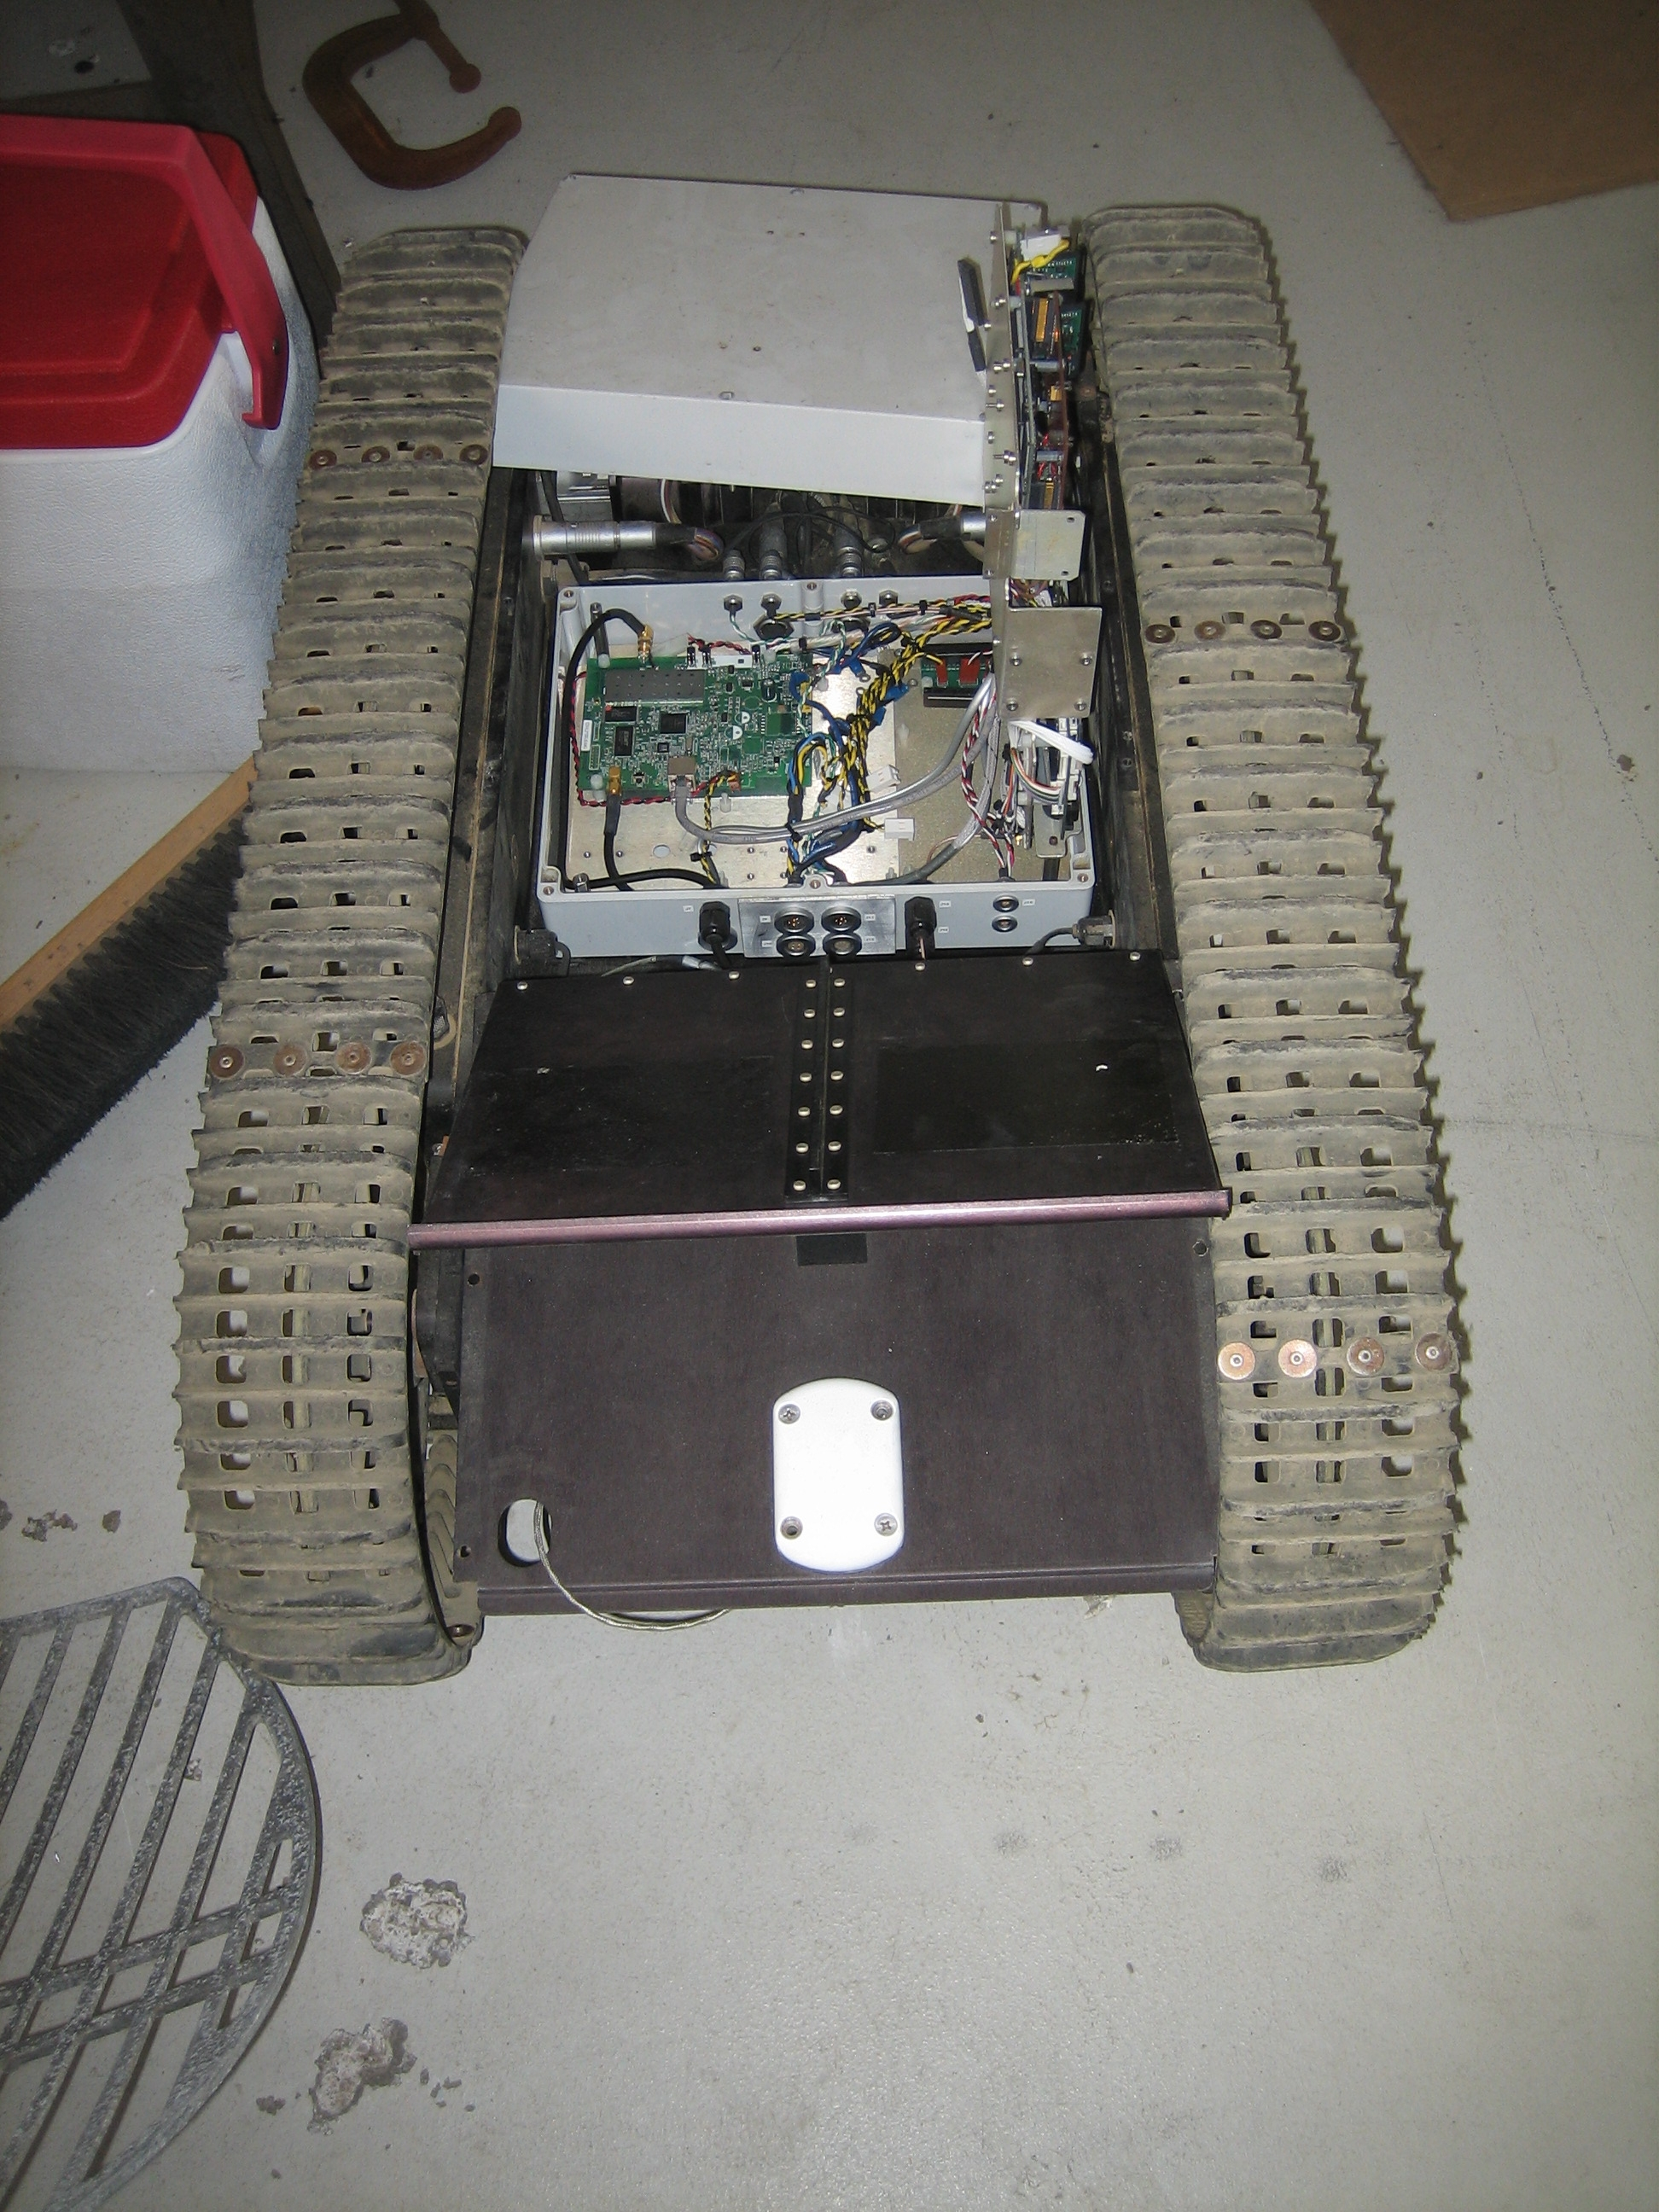
\includegraphics[width=.3\textwidth]{images/urbot}
	\caption{Urbot.}
	\label{fig:urbot}
\end{figure}

\section{MOCU \& JAUS}
\label{sec:mocujaus}
The Multi-Robot Operator Control Unit (MOCU) in Figure \ref{fig:mocu} is a highly configurable front-end for simultaneous command and control of multiple systems and was created at SPAWAR Systems Center, Pacific (SSCPAC) \cite{PowellMOCU08}. MOCU has the ability to use a variety of communications protocols for interfacing to different systems and uses the Joint Architecture for Unmanned Systems (JAUS) to send and receive data to all of the UGVs used in this research \cite{RoweJAUS08}. A combination of teleoperation using a joystick controller and autonomous navigation were used to collect data and test new ideas for estimation and controls. From within MOCU waypoints can be drawn on the overhead image and from those waypoints a route is generated and uploaded to the robot using the JAUS protocol. The robot will then attempt to drive that route autonomously and send back status information to MOCU using the controls and estimation code that is the focus of this research.

\begin{figure}[ht!]
	\centering
	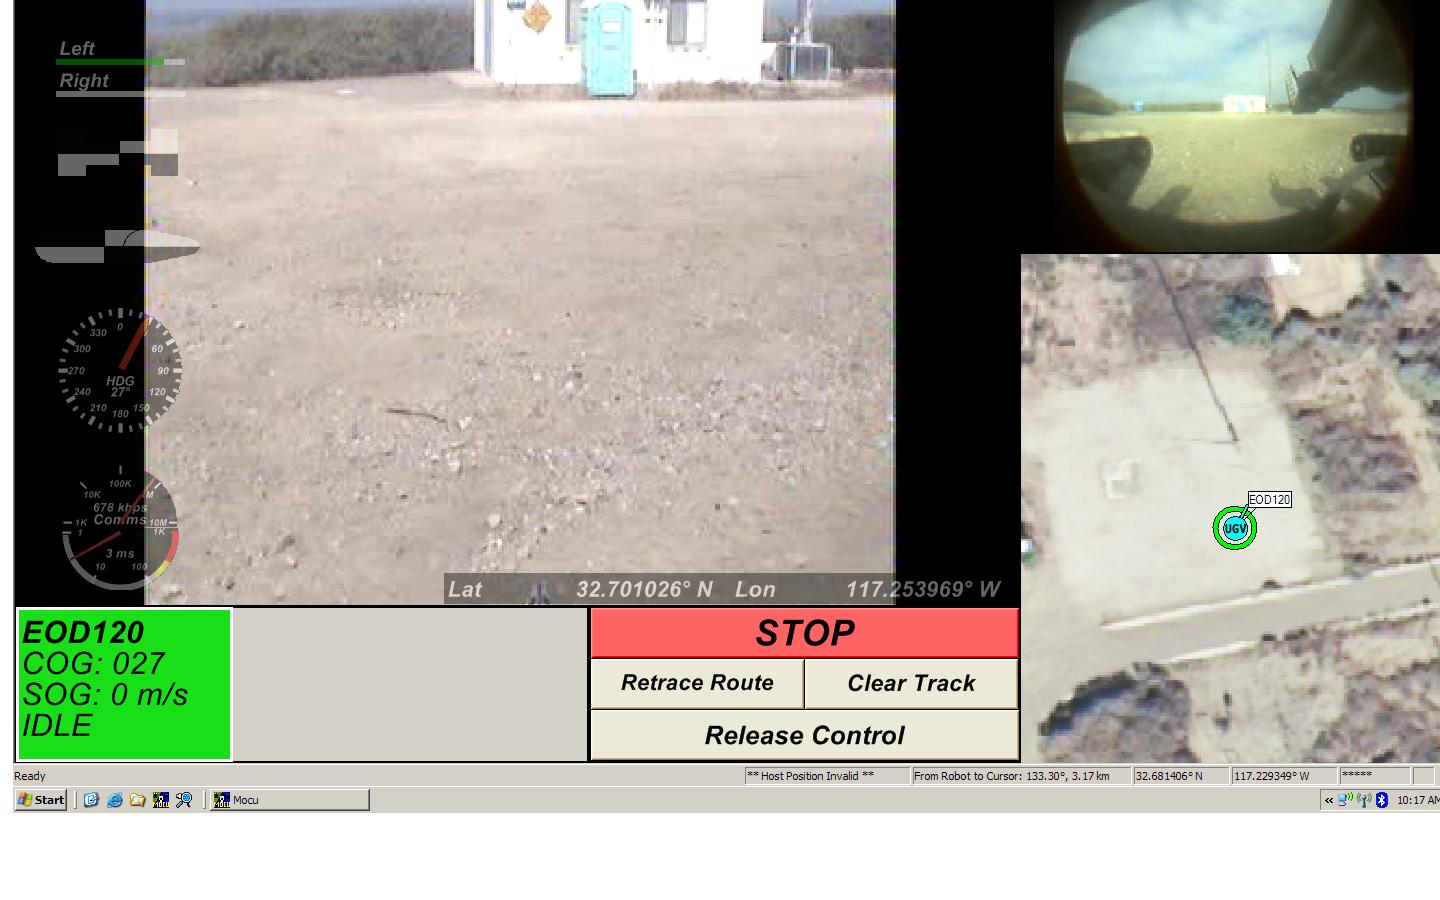
\includegraphics[width=.75\textwidth]{images/mocuPackbotScreenshot}
	\caption{Controlling PackBot with MOCU}
	\label{fig:mocu}
\end{figure}

\section{The Duals: Estimation \& Controls}
\label{sec:duals}
It is very difficult to simply work on either state estimation or controls individually as there is a large amount of coupling between the two areas. Although the main goal is to make the robots drive more smoothly and the actuator and motor outputs are ultimately generated by the control system it is still the case that the role of state estimation is equally important. If there exist large meaurement errors, drift or bias in the sensor readings then the robot will not have a very good idea of where it is locted and there will not be a controller that can stabilize the system. *** Talk about observability and controllability. Mention theory that shows link between estimation and control. ***

An example would be when the only sensor available for measurements is an IMU which suffers from drift and bias, where both effects are exagerrated by temperature. There have been situations in which an IMU was in a robot with the motors turned off so that the robot is not moving. However, due to excessive heat in the electronics box the IMU measurements report that the heading of the robot keeps moving in circles at a rate of $\frac{\pi}{5} rad/s$. With a controller that was known to keep the robot stable when the IMU was working properly started forcing the robot to turn in circles when the motors were turned on even though the command was to stay in one place. This shows the importance of state estimation on overall robot performance -- it is not enough to only have a good controller. A perfect controller will follow lousy estimates exactly and result in erratic behavior. Conversely, a poor controller will not output smooth trajectories even given perfect state estimates.

*** Work on a better explanation of how the two topics are linked and how I have attempted to separate the effects of one from the other in order to determine where efforts should be focused to best improve system performance. ***

\section{Sensors}
\label{sec:bgSensors}
The PackBot has its own computer that takes in commands for desired linear and angular velocities and outputs the correct motor controller commands. Typically the desired linear and angular velocity commands are generated by a user with a remote control. The research in this thesis used a set of sensors installed in one of the payload bays of the PackBot to determine which linear and angular velocity commands to send to the main PackBot computer without human intervention.

\subsection{Computer}
\label{sec:bgComputer}
The computer on the PackBot used for running the estimation and controls algorithms found in this thesis is the \href{http://www.beckhoff.com/english.asp?motherboards/cb4051.htm}{Beckhoff CB4051} with an Intel 2.0 GHz Core 2 Duo CPU.

\subsection{IMU}
\label{sec:bgIMU}
The IMU in the PackBot payload bay is a \href{http://www.microstrain.com/3dm-gx1.aspx}{Microstrain 3DM-GX1} that outputs Euler angles and angular rates.

\subsection{GPS}
\label{sec:bgGPS}
The GPS receiver in the PackBot payload by is a \href{http://www.novatel.com/products/gnss-receivers/oem-receiver-boards/oemv-receivers/}{Novatel OEMV}.

\subsection{Compass}
\label{sec:bgCompass}
Originally this sensor was not used on the PackBot but after initial testing it was determined that the heading reported by the Microstrain 3DM-GX1 was not very reliable and a \href{http://www.oceanserver-store.com/os3axdico3.html}{Ocean Server } compass was added to the PackBot payload bay.

\subsection{Wheel Encoders}
\label{sec:bgEncoders}
The PackBot is manufactured with wheel encoders that are read by the main PackBot computer and used to calculate a linear velocity and angular velocity that can be read by the payload computer when communicating with the main PackBot computer. Initially the wheel encoder data was not being used for backwards compatibility with other small UGVs that do not have wheel encoders but the systems that do not have wheel encoders are no longer used by EOD groups so that data has been incorporated into the sensor suite used by the algorithms in this thesis.
